%!TEX root = presentation.tex
\section{Introduction}

\subsection{Contexte}
\begin{frame}{}

{\small 
	\begin{minipage}{.3\textwidth}
		\centering
		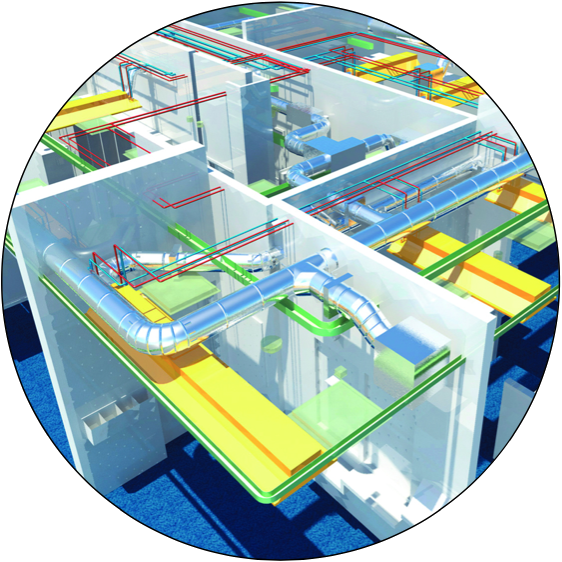
\includegraphics[width=\textwidth]{img/bim2.png}\\
		Building Information Modeling (BIM)
	\end{minipage}
	\hfill
	\begin{minipage}{.3\textwidth}
		\centering
		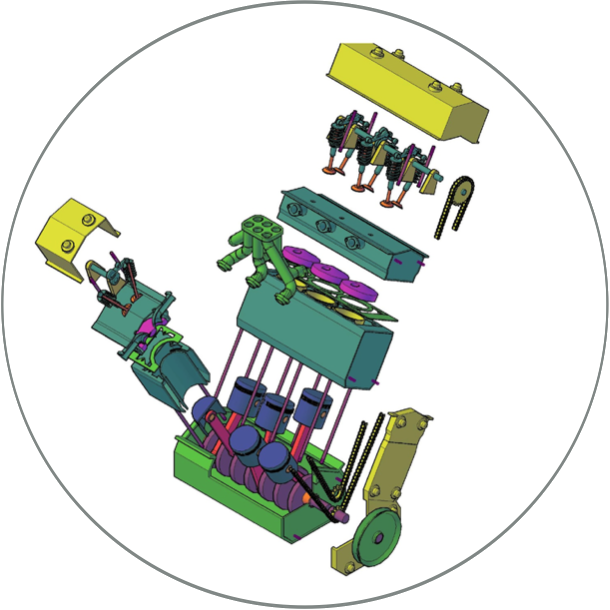
\includegraphics[width=\textwidth]{img/cad2.png}\\
		Conception Assistée par Ordinateur (CAO)
	\end{minipage}
	\hfill
	\begin{minipage}{.3\textwidth}
		\centering
		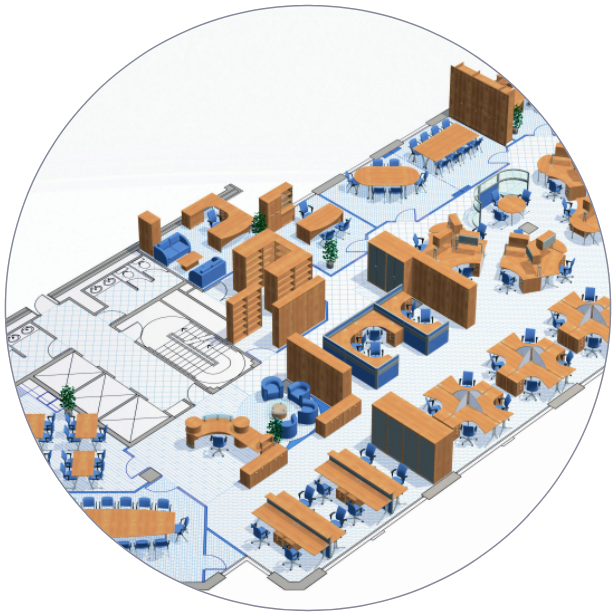
\includegraphics[width=\textwidth]{img/spaceplanning2.png}\\
		Aménagement \\ d'espace
	\end{minipage}}
	\vspace*{0.5cm}
	\centering
	
	Collaborer de manière distante sur une scène 3D
\end{frame}

%\begin{frame}{Besoins pour collaborer}
%Accompagner un groupe de 
%participants dans la réalisation d'une tâche en fournissant une 
%interface vers un environnement partagé :
%\begin{itemize}
%	\item coordination 
%	%: harmonisation des tâches, des rôles et du calendrier dans 
%	%un système simple
%	\item coopération 
%	%: résoudre des problèmes dans des environnements 
%	%complexes (impossible seul ou beaucoup plus efficace à plusieurs)
%\end{itemize}
%%Collaboration centrée activité \cite{Gotta2007} et par équipe 
%%\cite{Callahan2008}.
%
%Utilisation d'un Système d'Edition Collaborative (SEC) en temps-réel sur un 
%document (3D)
%
%Maintien de la cohérence et respect de l'intention
%%Un SEC en temps réel permet à plusieurs utilisateurs de 
%%visualiser et d'éditer de manière simultanée le même document (texte, image, 
%%objet 3D)
%
%EVC3D : réseau + systèmes distribués + 3D + interface utilisateur
%\end{frame}



\subsection{Problématique}

\begin{frame}{}
	\begin{textblock*}{95mm}(3.3cm,0.5\textheight)
		\centering \large
		\textbf{ {\color{Purple}Comment engager toutes les ressources \\ à 
		disposition 
		lors de la collaboration  sur le web?}}
	\end{textblock*}
\end{frame}



\subsection{État de l'art}


\begin{frame}
\centering

\only<1>{
	\inputTikZ{1.1}{img/tikz/namewithpics.tex}
}
\only<2>{
	\inputTikZ{1.1}{img/tikz/conception3D.tex}
}

\only<3>{
	\inputTikZ{1.1}{img/tikz/archcomm.tex}
}

\only<4>{
	\inputTikZ{1.1}{img/tikz/tracabilite.tex}
}

\only<5>{
	\inputTikZ{1.1}{img/tikz/allwithpics.tex}
}
\end{frame}


\begin{frame}{}
\renewcommand{\baselinestretch}{0.9} 
\begin{textblock*}{65mm}(8mm,0.15\textheight)
	\only<1->{
	\begin{exampleblock}{\centering Q1}
		\centering \small	
		Quelle \textbf{architecture réseau} propose une gestion efficace,  robuste et 
		temps 
réel des données 3D dans un environnement \textbf{web}?
	\end{exampleblock}}
\end{textblock*}

\begin{textblock*}{65mm}(90mm,0.15\textheight)
	\only<2->{
	\begin{exampleblock}{\centering Q2}
		\centering \small 
		Quelle architecture logicielle confère une \textbf{traçabilité} des 
	données conforme aux règles métiers liées à la manipulation d'objets 3D ?
	\end{exampleblock}}
\end{textblock*}

\begin{textblock*}{60mm}(10mm,0.65\textheight)
	\only<3->{
	\begin{exampleblock}{\centering Q3}
		\centering \small 
		Quels sont les mécanismes assurant à l'utilisateur d'être \textbf{autonome} 
		tout en 
		collaborant ?
	\end{exampleblock}}
\end{textblock*}

\begin{textblock*}{60mm}(93mm,0.65\textheight)
	\only<4->{
	\begin{exampleblock}{\centering Q4}
		\centering \small 
		Comment garantir le \textbf{respect des règles métiers} liées à la 
		manipulation 
		d'objets 3D lors de l'implantation?
	\end{exampleblock}}
\end{textblock*}

\begin{textblock*}{70mm}(48mm,0.9\textheight)
	\only<5->{
	\begin{exampleblock}{\centering Q5}
		\centering \small 
		Quelles sont les \textbf{critères} permettant d'évaluer un tel système de 
		manière quantitative ? qualitative ? 
	\end{exampleblock}}
\end{textblock*}

\begin{textblock*}{95mm}(3.3cm,0.5\textheight)
	\centering \large
	\textbf{ {\color{Purple}Comment engager toutes les ressources \\ à disposition 
			lors de la collaboration sur le web ?}}
\end{textblock*}

\end{frame}

